\begin{figure}
  \centering
  \begin{tikzpicture}    
    \node at (10, 0) {
      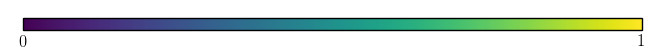
\includegraphics[height=4.2cm]{experiments/3d/vae_occ/easy_15/colorbar}
    };
    
    \node at (0, 0){
      \includegraphics[width=6cm]{experiments/shapenet/vae_occ_aml/hard_15_long_statistics_75/results_0}
    };
    
    \node at (6.5, 0){
      \includegraphics[width=6cm]{experiments/shapenet/vae_occ_aml/hard_15_long_statistics_75/results_3}
    };
    
    \draw[-,dashed](-3.5,-2.15) -- (10,-2.15);
    
    % --- 
    \node at (0, -3.5){
      \includegraphics[width=6cm]{experiments/shapenet/baseline/hard_15/results_0}
    };
    
    \node at (6.5, -3.5){
      \includegraphics[width=6cm]{experiments/shapenet/baseline/hard_15/results_3}
    };
    
    \node[rotate=90] at (-3.5, -3.5) {Baseline};
    \node[rotate=90] at (-3.5, 0) {\AML};
    %\node at (3.25, 2.5) {reconstruction};
  \end{tikzpicture}
  \vskip 6px
  
  % TODO short caption
  \caption{Qualitative results of \AML for \hard difficulty of the ShapeNet
  dataset. We show results for occupancy only in comparison with the supervised
  baseline. On top, we show horizontal slices of the volumes
  corresponding to the observed points, the partial free space, the target
  shape, the predicted shape and the corresponding error. On the bottom,
  \ie for the baseline, we only show the target shape, the predicted shape
  and the corresponding error. Again, we show heights $8 + 2i$ for
  $0 \leq i < 8$. 3D visualizations of these results can be found
  in Figure \ref{fig:experiments-shapenet-aml-qual-2}.}
  \label{fig:experiments-shapenet-aml-qual-1}
\end{figure}
\begin{figure}
  \centering
  \hspace*{-1cm}
  \begin{tikzpicture}
    \node at (0, 0) {
      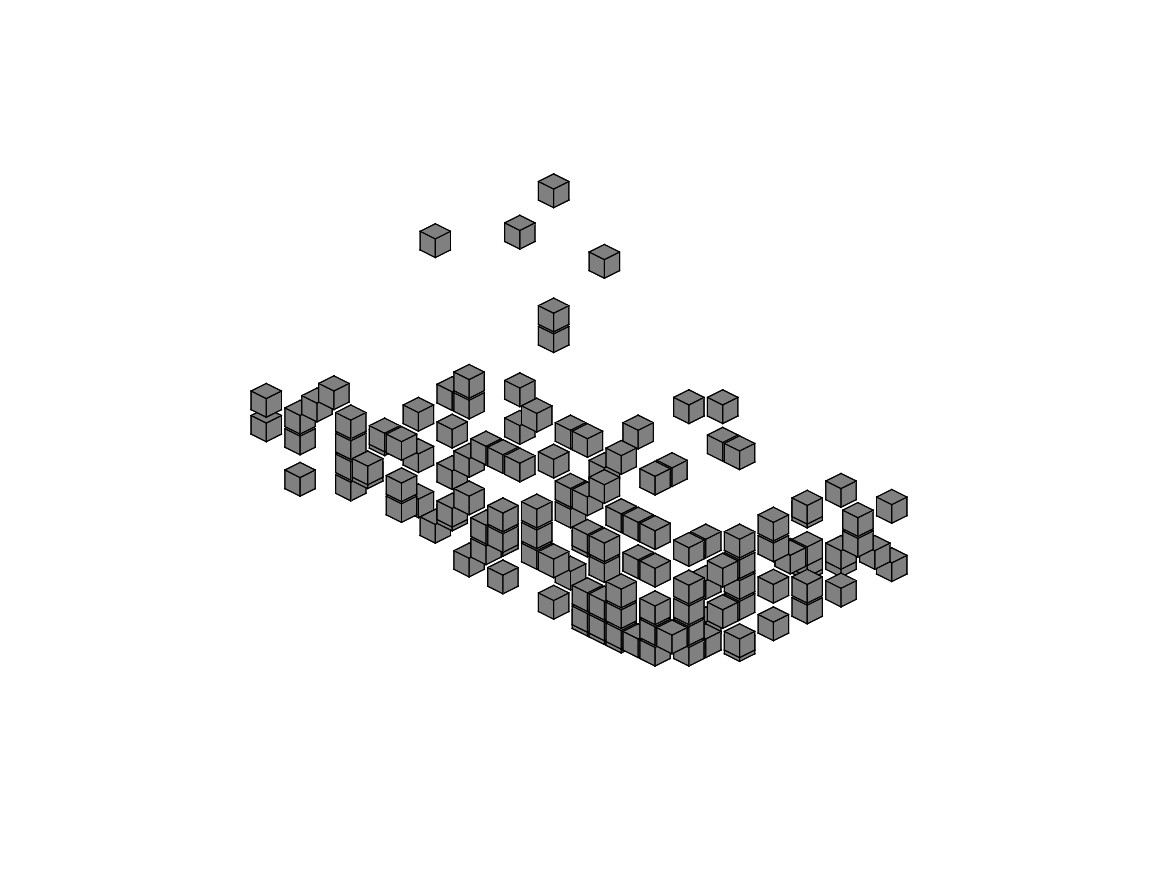
\includegraphics[width=3.75cm,trim={3.5cm 2.5cm 3.5cm 2.5cm},clip]{experiments/shapenet/vae_occ_aml/hard_15_long_statistics_75/0_input_45}
    };
    \node at (3.5, 0) {
      \includegraphics[width=3.75cm,trim={3.5cm 2.5cm 3.5cm 2.5cm},clip]{experiments/shapenet/vae_occ_aml/hard_15_long_statistics_75/0_prediction_45}
    };
    \node at (7, 0) {
      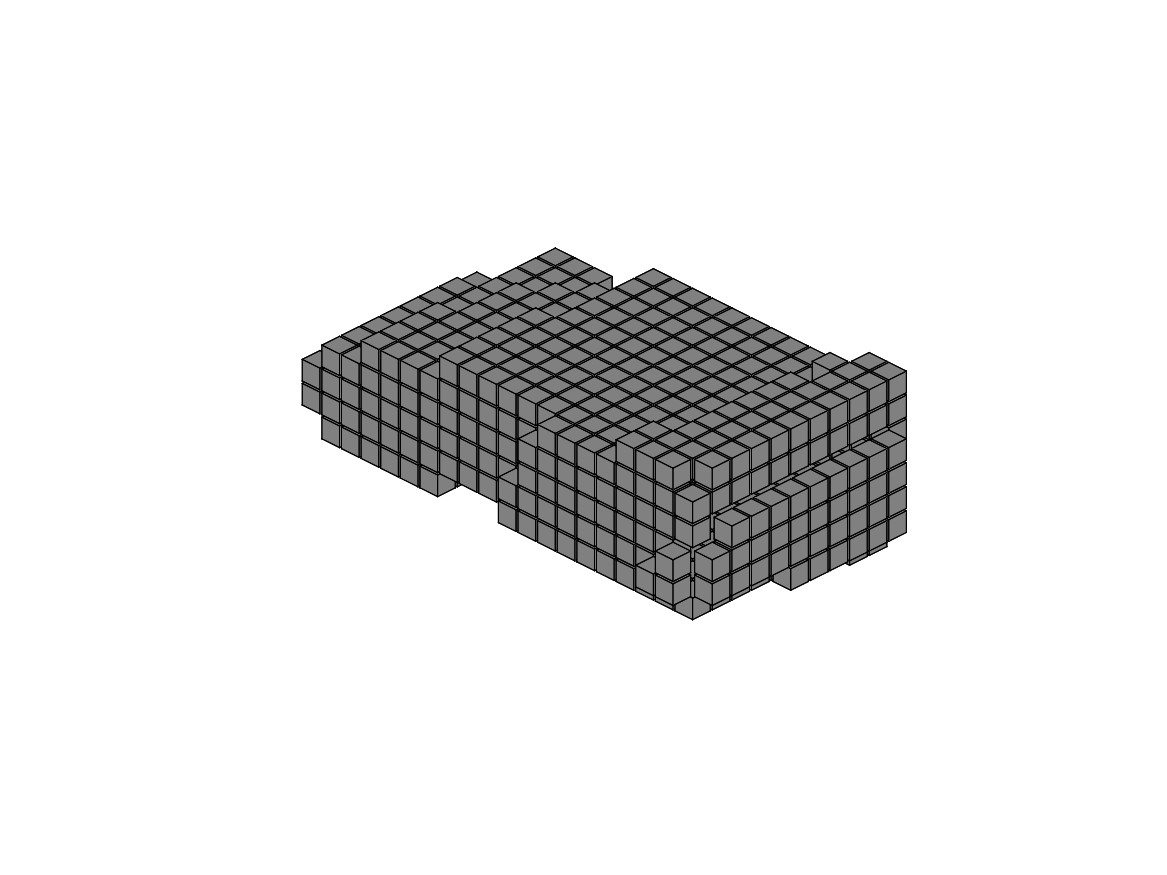
\includegraphics[width=3.75cm,trim={3.5cm 2.5cm 3.5cm 2.5cm},clip]{experiments/shapenet/vae_occ_aml/hard_15_long_statistics_75/0_target_45}
    };
    \node at (10.5, 0) {
      \includegraphics[width=3.75cm,trim={3.5cm 2.5cm 3.5cm 2.5cm},clip]{experiments/shapenet/baseline/hard_15/0_prediction_45}
    };
    
    \node at (0, -3) {
      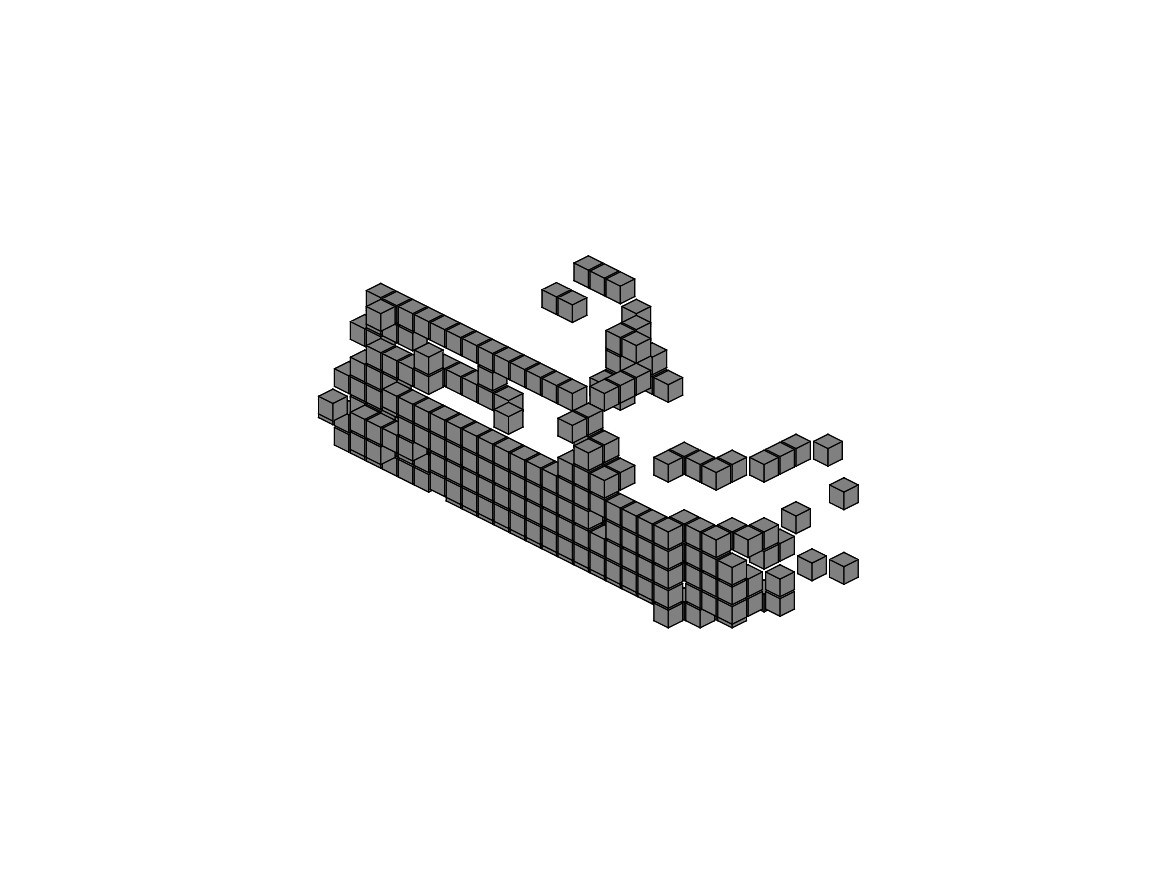
\includegraphics[width=3.75cm,trim={3.5cm 2.5cm 3.5cm 2.5cm},clip]{experiments/shapenet/vae_occ_aml/hard_15_long_statistics_75/3_input_45}
    };
    \node at (3.5, -3) {
      \includegraphics[width=3.75cm,trim={3.5cm 2.5cm 3.5cm 2.5cm},clip]{experiments/shapenet/vae_occ_aml/hard_15_long_statistics_75/3_prediction_45}
    };
    \node at (7, -3) {
      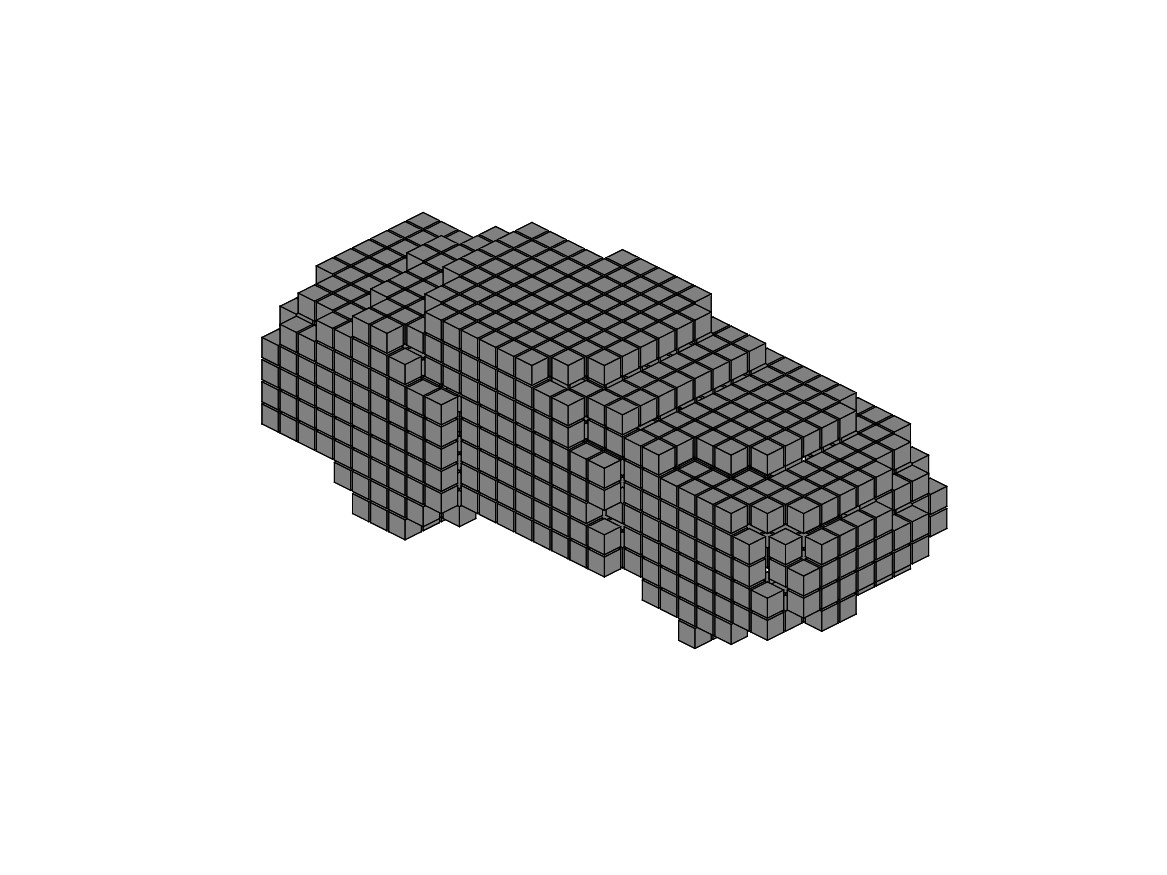
\includegraphics[width=3.75cm,trim={3.5cm 2.5cm 3.5cm 2.5cm},clip]{experiments/shapenet/vae_occ_aml/hard_15_long_statistics_75/3_target_45}
    };
    \node at (10.5, -3) {
      \includegraphics[width=3.75cm,trim={3.5cm 2.5cm 3.5cm 2.5cm},clip]{experiments/shapenet/baseline/hard_15/3_prediction_45}
    };
    
    \node at (0, 1.75) {Input};
    \node at (3.5, 1.75) {\AML};
    \node at (7, 1.75) {Baseline};
    \node at (10.5, 1.75) {Target};
  \end{tikzpicture}
  \caption{3D visualizations for comparing \AML and the supervised baseline
  on \hard difficulty of the ShapeNet dataset. Results were obtained using occupancy
  only. As can be seen, \AML has difficulties with the roofs; additionally,
  the first example occurs to the predicted with flipped orientation as our
  ShapeNet dataset also includes flipped variants.}
  \label{fig:experiments-shapenet-aml-qual-2}
\end{figure}
\begin{figure}
  \centering
  \begin{tikzpicture}    
    \node at (-3.5,0) {
      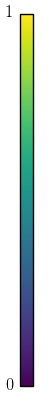
\includegraphics[height=4.25cm]{experiments/3d/vae_occ_sdf/colorbar_0}
    };
    
    \node at (0, 0){
      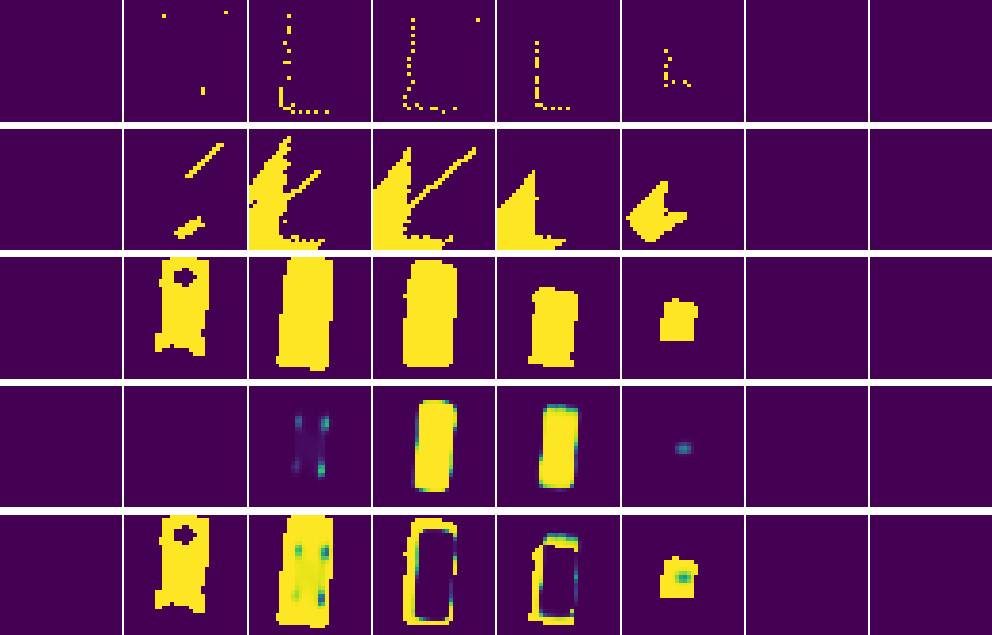
\includegraphics[width=6cm]{experiments/shapenet/vae_occ_sdf_aml/hard_15_statistics/results_0_0}
    };
    \node at (0, -4){
      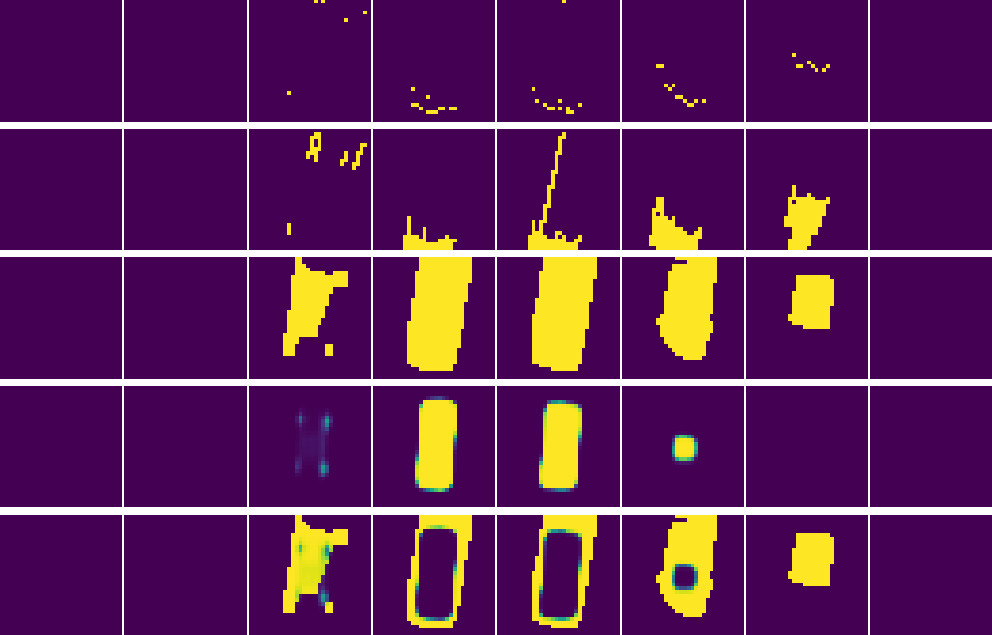
\includegraphics[width=6cm]{experiments/shapenet/vae_occ_sdf_aml/hard_15_statistics/results_3_0}
    };
    
    \node at (6.5, 0){
      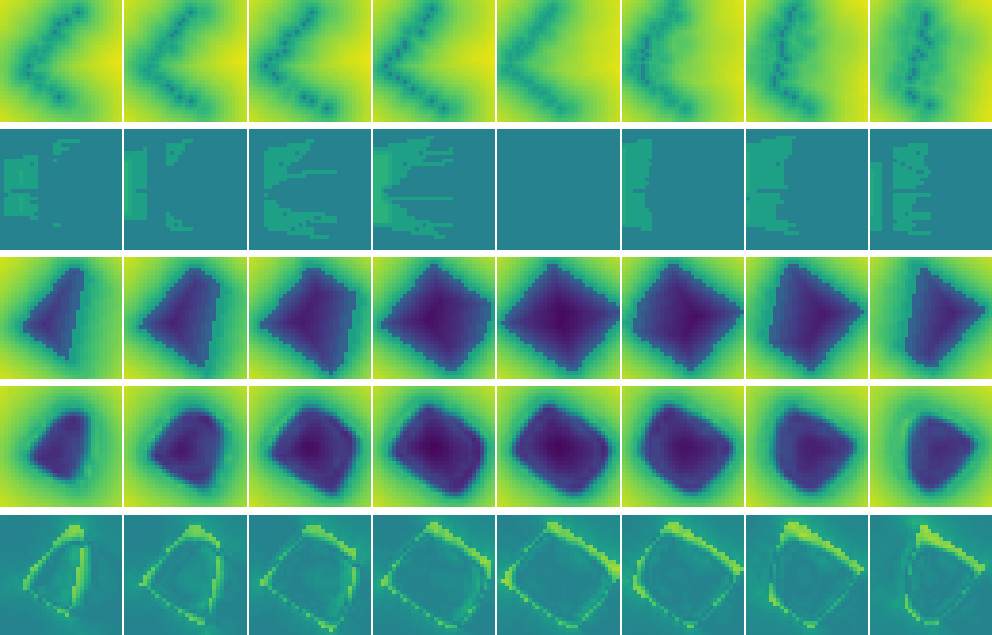
\includegraphics[width=6cm]{experiments/shapenet/vae_occ_sdf_aml/hard_15_statistics/results_0_1}
    };
    \node at (6.5, -4){
      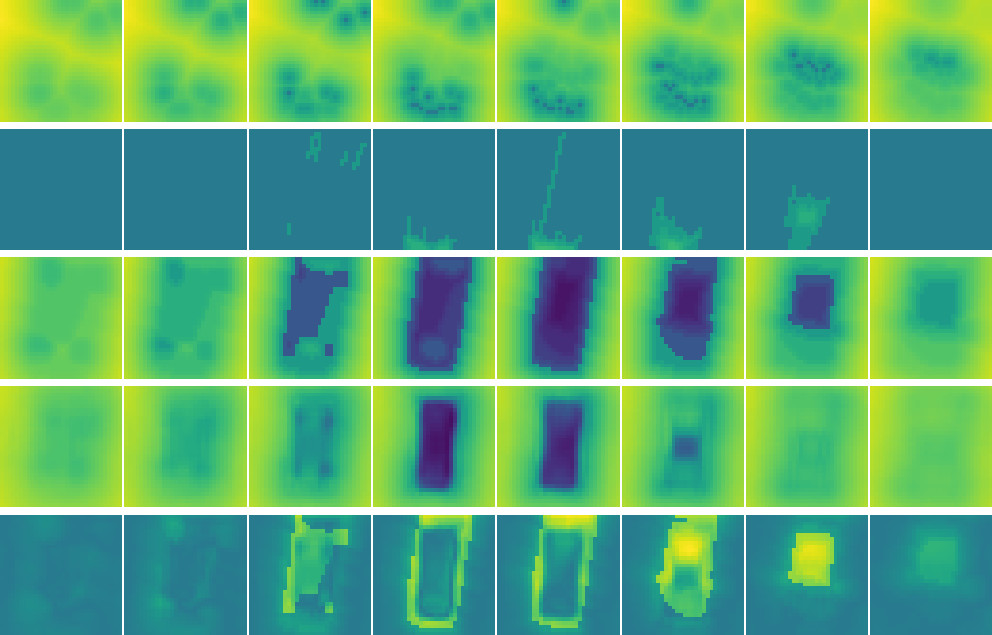
\includegraphics[width=6cm]{experiments/shapenet/vae_occ_sdf_aml/hard_15_statistics/results_3_1}
    };
    
    \node at (10,0) {
      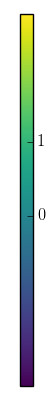
\includegraphics[height=4.25cm]{experiments/3d/vae_occ_sdf/colorbar_1}
    };
    
    \node at (0, 2.25) {occupancy};
    \node at (6.5, 2.25) {signed distance function};
  \end{tikzpicture}
  \vskip 6px

  % TODO short caption
  \caption{Qualitative results for \AML using both occupancy and signed distance
  functions. We show two examples from the \hard dataset for both modalities.
  In both cases we show slices of the volumes corresponding to the observed points,
  the partial free space, the target shape as well as the predicted shape and its
  error. Again, we show heights $8 + 2i$ for $0 \leq i < 8$. Triangular meshes
  corresponding the the predicted signed distance functions can be found
  in Figure \ref{fig:experiments-shapenet-aml-qual-4}.}
  \label{fig:experiments-shapenet-aml-qual-3}
\end{figure}
\begin{figure}
  \centering
  \begin{tikzpicture}
    \node at (0, 0) {
      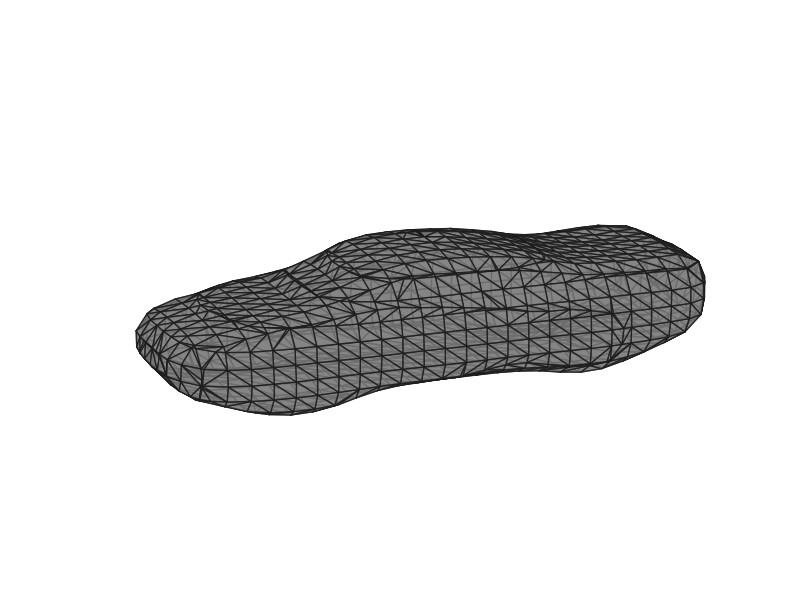
\includegraphics[width=2.75cm,trim={1cm 2cm 1cm 2cm},clip]{experiments/shapenet/vae_occ_sdf_aml/hard_15_statistics/0_prediction}
    };
    \node at (3, 0) {
      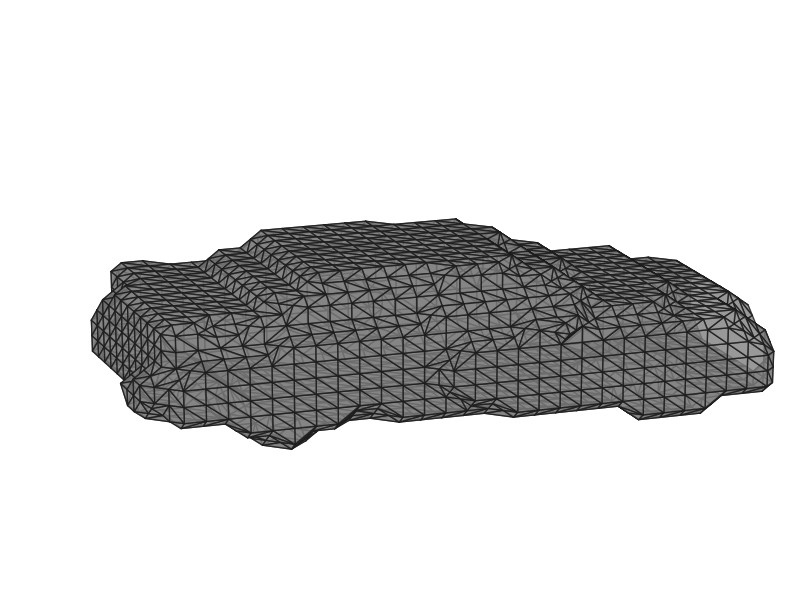
\includegraphics[width=2.75cm,trim={1cm 2cm 1cm 2cm},clip]{experiments/shapenet/vae_occ_sdf_aml/hard_15_statistics/0_target}
    };
    
    \draw[-,dashed] (5,-1) -- (5, 1);
    
    \node at (7, 0) {
      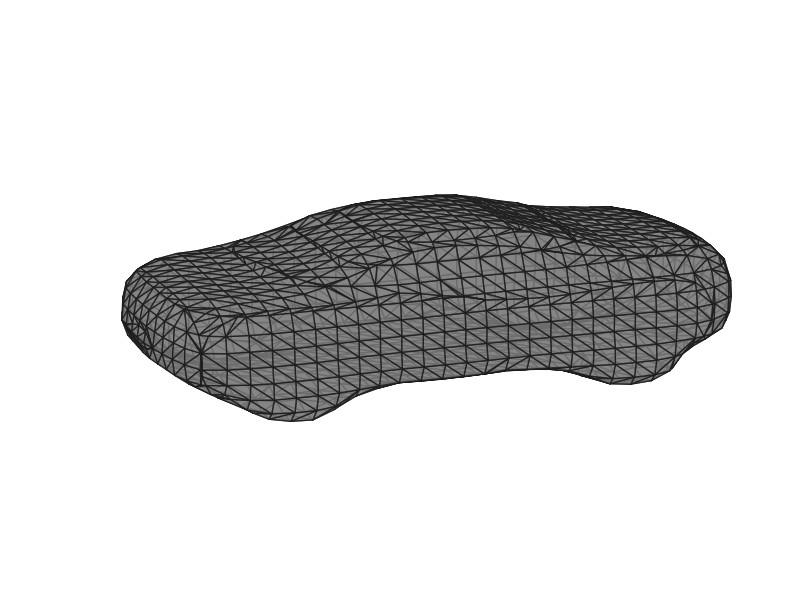
\includegraphics[width=2.75cm,trim={1cm 2cm 1cm 2cm},clip]{experiments/shapenet/vae_occ_sdf_aml/hard_15_statistics/3_prediction}
    };
    \node at (10, 0) {
      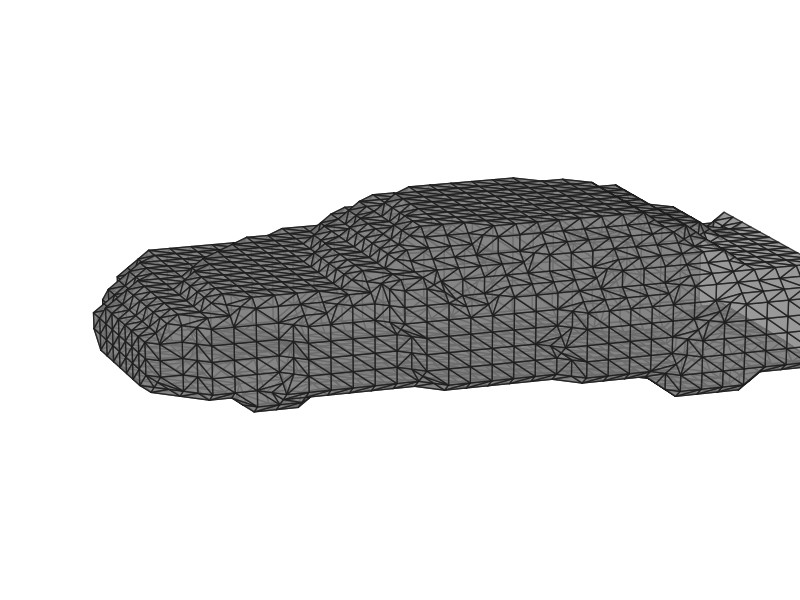
\includegraphics[width=2.75cm,trim={1cm 2cm 1cm 2cm},clip]{experiments/shapenet/vae_occ_sdf_aml/hard_15_statistics/3_target}
    };
    
    \node at (0, 1) {\AML};
    \node at (3, 1) {Target};
    \node at (7, 1) {\AML};
    \node at (10, 1) {Target};
  \end{tikzpicture}
  \caption{Qualitative results for \AML after using marchign cubes to
  derive meshes from the predictions and the targets. For the targets, we can
  clearly see that the used signed distance functions are derived from the
  occupancy grids. The predictions, in contrast a re more smooth, however,
  consistently underestimate the size of the car.}
  \label{fig:experiments-shapenet-aml-qual-4}
\end{figure}
